\documentclass[red]{tutorial}



\usepackage[no-math]{fontspec}
\usepackage{xpatch}
	\renewcommand{\ttdefault}{ul9}
	\xpatchcmd{\ttfamily}{\selectfont}{\fontencoding{T1}\selectfont}{}{}
	\DeclareTextCommand{\nobreakspace}{T1}{\leavevmode\nobreak\ }
\usepackage{polyglossia} % English please
	\setdefaultlanguage[variant=us]{english}
%\usepackage[charter,cal=cmcal]{mathdesign} %different font
%\usepackage{avant}
\usepackage{microtype} % Less badboxes



\usepackage[charter,cal=cmcal]{mathdesign} %different font
%\usepackage{euler}
 
\usepackage{blindtext}
\usepackage{calc, ifthen, xparse, xspace}
\usepackage{makeidx}
\usepackage[hidelinks, urlcolor=blue]{hyperref}   % Internal hyperlinks
\usepackage{mathtools} % replaces amsmath



\usepackage{bbm} %lower case blackboard font
\usepackage{amsthm, bm}
\usepackage{thmtools} % be able to repeat a theorem
\usepackage{thm-restate}
\usepackage{graphicx}
\usepackage{xcolor}
\usepackage{multicol}
\usepackage{fnpct} % fancy footnote spacing

 
\newcommand{\xh}{{{\mathbf e}_1}}
\newcommand{\yh}{{{\mathbf e}_2}}
\newcommand{\zh}{{{\mathbf e}_3}}
\newcommand{\R}{\mathbb{R}}
\newcommand{\Z}{\mathbb{Z}}
\newcommand{\N}{\mathbb{N}}
\newcommand{\Perp}{\mathrm{perp}}
\newcommand{\Span}{\mathrm{span}\,}
\newcommand{\Img}{\mathrm{img}\,}
\newcommand{\Null}{\mathrm{null}\,}
\newcommand{\Range}{\mathrm{range}\,}
\newcommand{\rref}{\mathrm{rref}}
\newcommand{\Rank}{\mathrm{rank}}
\newcommand{\nnul}{\mathrm{nullity}}
\newcommand{\mat}[1]{\begin{bmatrix}#1\end{bmatrix}}
\newcommand{\chr}{\mathrm{char}}
\renewcommand{\d}{\mathrm{d}}


\theoremstyle{definition}
\newtheorem{example}{Example}[section]
\newtheorem{defn}{Definition}[section]

%\theoremstyle{theorem}
\newtheorem{thm}{Theorem}[section]

\pgfkeys{/tutorial,
	name={Tutorial 3},
	author={Jason Siefken \& Bernardo Galv\~ao-Sousa},
	course={MAT 244},
	date={},
	term={},
	title={Modelling with Parametres}
	}

\begin{document}
	\begin{tutorial}
				\begin{objectives}
			In this tutorial you will explore the Lotka-Volterra model in more detail.

	These problems relate to the following Course Learning Objectives:
			\textit{
Interpret and analyze models based on differential equations using tools like simulation, phase
portraits, analysis of stability, and linear approximation.
			}
		\end{objectives}

\subsection*{Problems}

Consider the Predator-Prey Lotka-Volterra model (the LV model) with unknown parameters:
\begin{align*}
	F' &= a \cdot R\cdot F - b \cdot F \\
	R' &= c \cdot R - d \cdot R \cdot F
\end{align*}
and $a,b,c,d\geq 0$. 

\begin{enumerate}
	\item In class, we used the parameters $a=0.01, b=1.1, c=1.1, d=0.1$.

	\begin{enumerate}
		\item	Make a phase portrait for the LV model on Desmos 
			using the parameters from class.

		\url{https://www.desmos.com/calculator/vrk0q4espx}

		\item The arrows point in the clockwise direction. What would
			it mean if the arrows pointed in the
			\emph{counter-clockwise} direction? Explain in terms 
			of Rabbits and Foxes. Would this be realistic?
	\end{enumerate}

	\item\label{qual}
		Using the parameters from class, the rabbit and fox populations 
		evolve \emph{periodically}. In this case, all
		solutions share the same \emph{qualitative}
		behaviour (namely they are periodic).

		\begin{enumerate}
			\item Analyze your phase portrait for different values of $a,b,c,d$ until you
				find parameters that look like they give rise to a different
				qualitative behaviour.
			\item Simulate (using Euler's method in a spreadsheet) some
				solutions that exhibit different qualitative
				behaviour.
			\item Tell a story about the fox and rabbit population for
				the different parameters you came up with.
		\end{enumerate}
		
		\item If $a,b,c,d>0$, the maximum rabbit population always
			occurs when there are $c/d$ foxes.
		\begin{enumerate}
			\item Justify this claim. (Make sure your justification references the equations.)
			\item Find a similar condition for when the foxes are at their maximum population.
			\item Find conditions for when neither the rabbit nor the fox populations change.
			\item If we relax the conditions to $a,b,c,d\geq 0$, are your conditions still valid?
				Can your work in this question be used to explain when you should
				expect different qualitative behaviour of solutions (i.e., what
				you worked on in part \ref{qual})?
		\end{enumerate}

%		\item From the phase plane, how can you identify the maximum number of foxes/rabbits? What about the minimum?
%		\item Find a formula for the maximum and minimum number of foxes and rabbits. \\
%		
%
%		\item Using an implicit derivative, calculate $\frac{dF}{dR}$ as a function of $F$ and $R$. Solve the separable differential equation.
%				$$
%				-b \ln(y)+ay +dx-c\ln(x) = {\rm Constant}
%				$$
%		\item This means that the graphs of solutions in the phase plane, are level sets of a function $\Psi(x,y)$. What is this function $\Psi(x,y)$?
%		\item Use this fact to find a formula for the max/min of the number of rabbits/foxes that depend only on the initial conditions $r_0$ and $f_0$ (and on the constants $a,b,c,d$).
		
		

	
	
		
\end{enumerate}

	\end{tutorial}

	\begin{solutions}
				\begin{enumerate}
			\item \begin{enumerate}
				\item \phantom{x}
				
				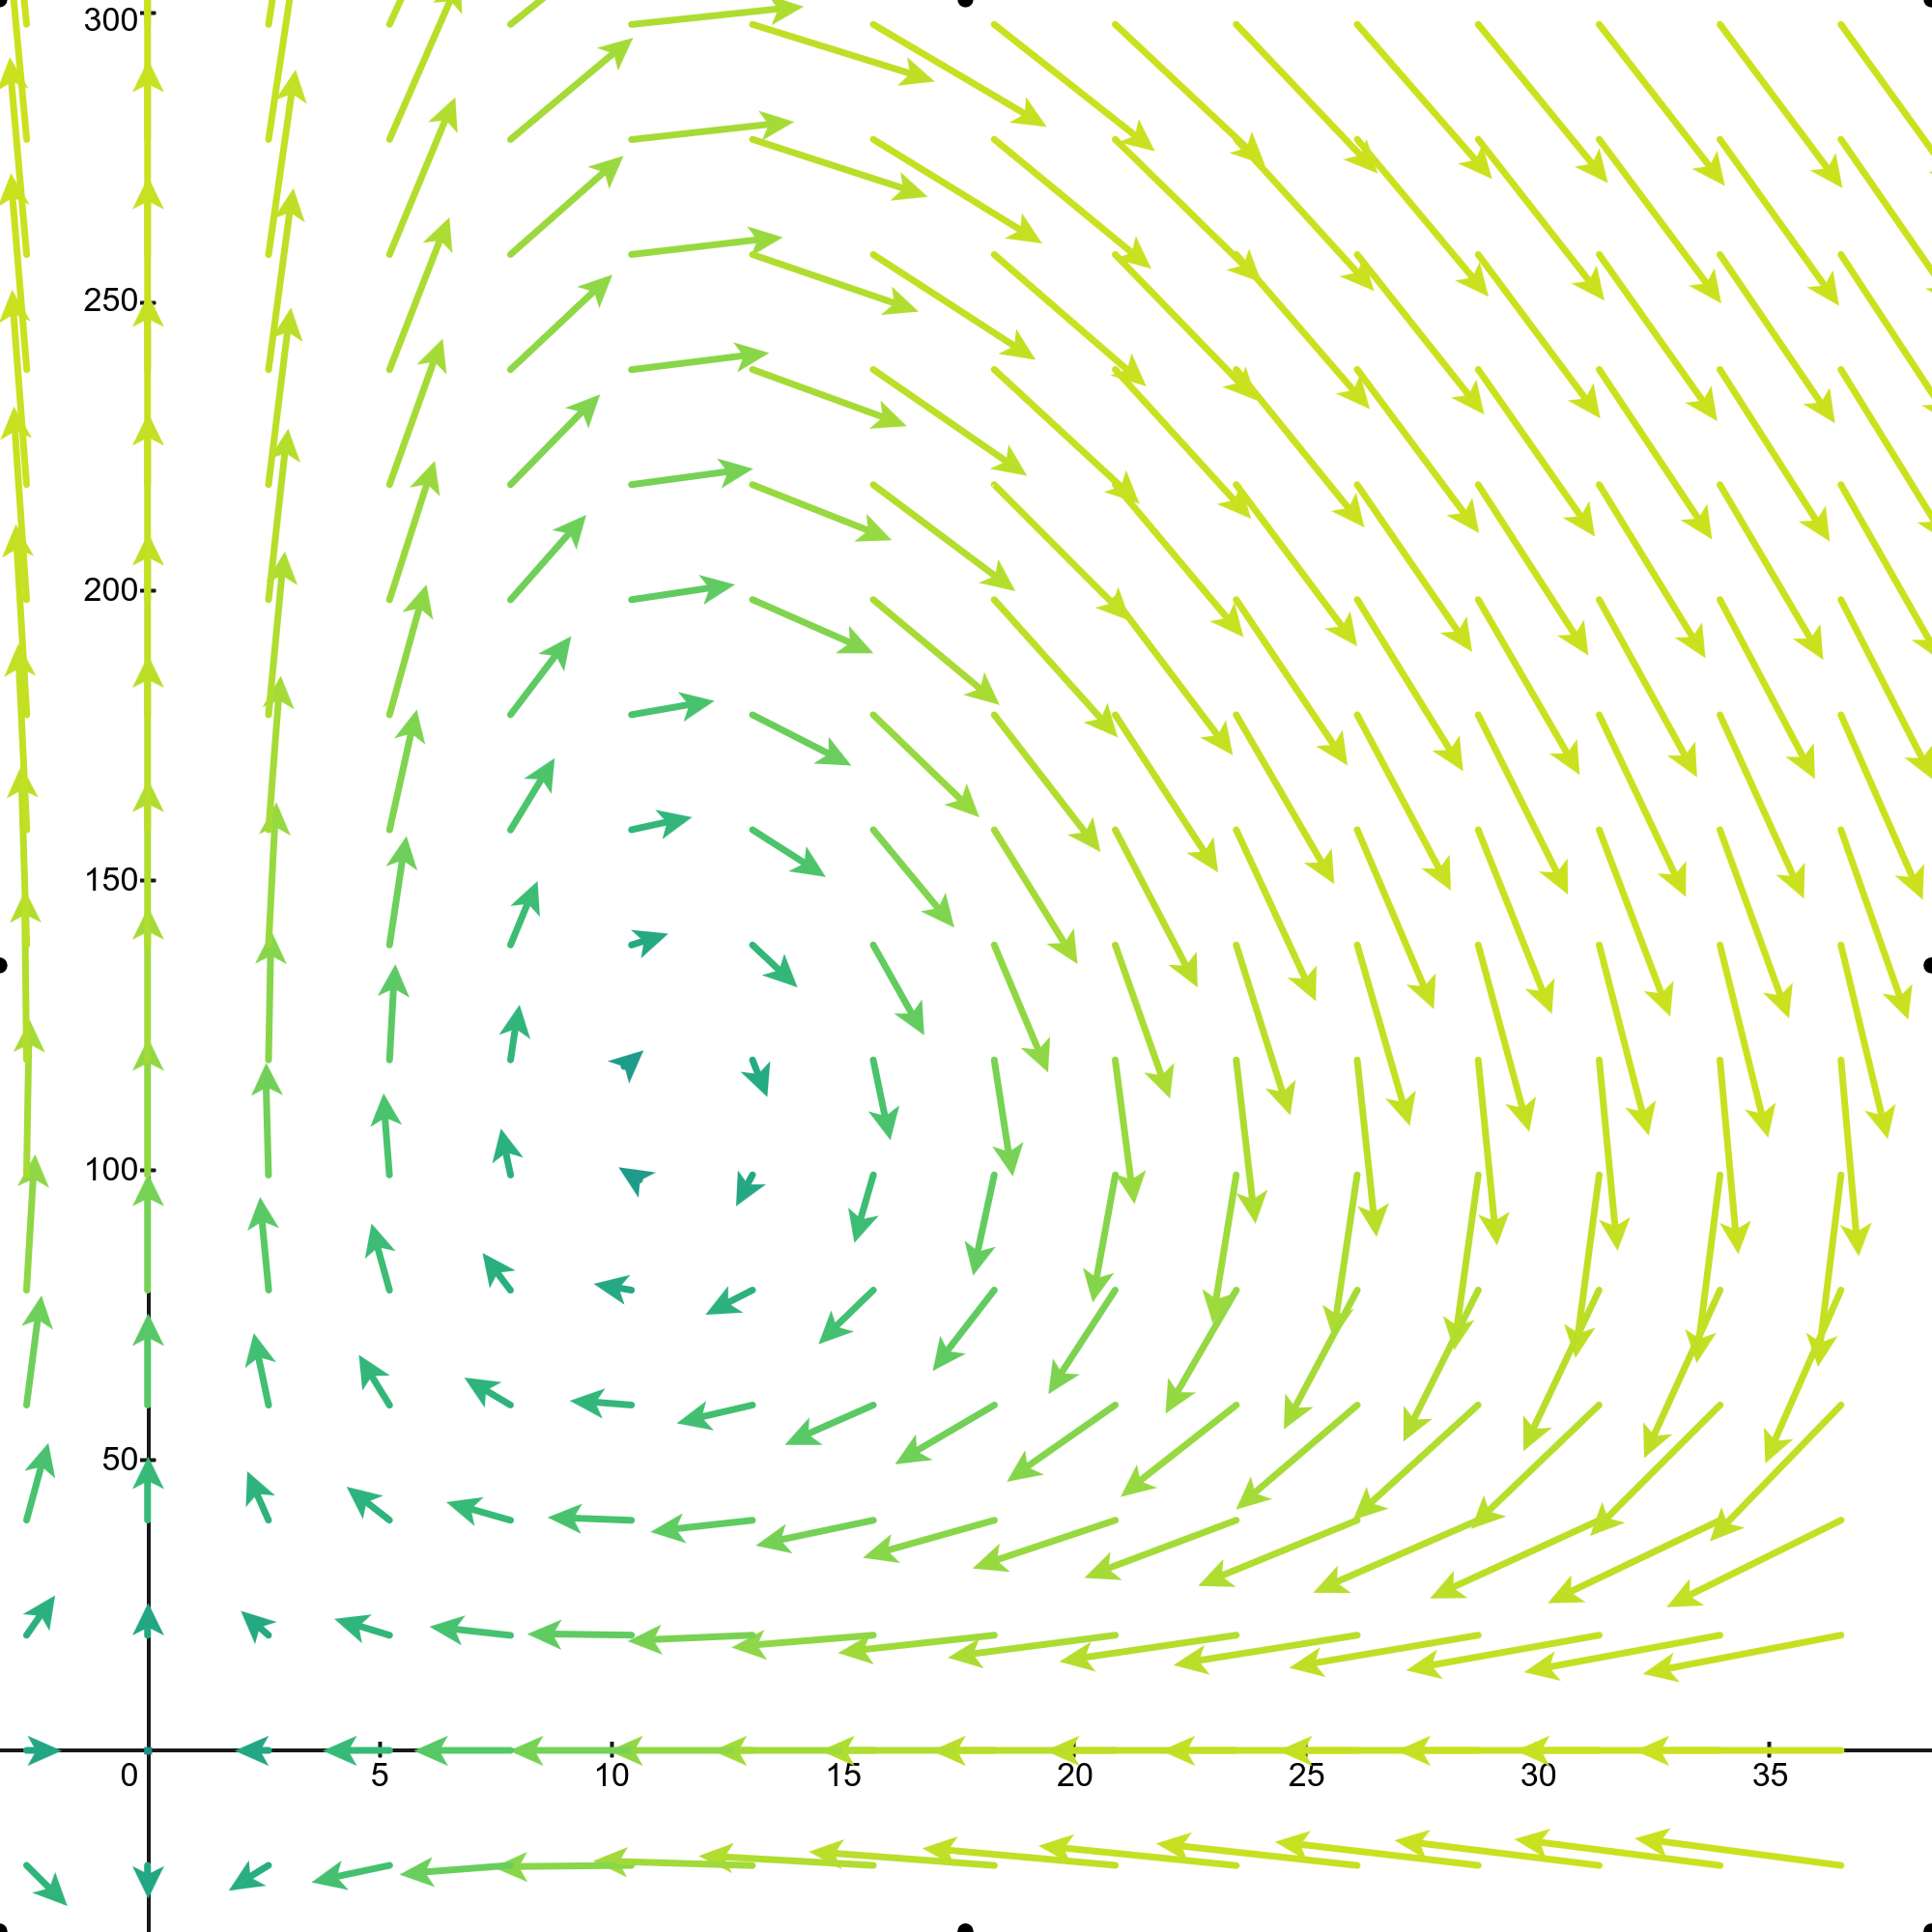
\includegraphics[width=3in]{resources/tutorial-02-1a.png}

				\item Arrows to the right of $F=11$ point down. That means as there are more foxes, the rabbit population decreases.
				Arrows to the left of $F=11$ point up, so as there are fewer foxes, there are more rabbits. If the arrows were oriented in the opposite direction,
				more foxes would lead to more rabbits, which is the opposite of what we would expect if the foxes ate the rabbits.
			\end{enumerate}
			\item \begin{enumerate}
				\item As long as $a,b,c,d>0$, there will be periodic behaviour.
				However, if any of the parameters becomes zero, the behaviour will change.
				\item 
				\item If we leave $a,c,d$ as they are and set $b$ to zero, the foxes will never die.
				Thus, the fox population will grow and grow as long as there are rabbits available. However,
				once the foxes eat the rabbits to extinction, they fox population will be unchanged, since the foxes are
				immortal!
			\end{enumerate}
			\item \begin{enumerate}
				\item We know that a maximum rabbit population occurs when $R'=0$. Manipulating the equation for
				$R'$, we find that $R'=0$ when $F=c/d$.
				\item Manipulating the equation for $F'$, we find that $F'=0$ when $R=b/a$.
				\item If neither populations change, then we must have $F'=0$ and $R'=0$. This occurs when
				$(F,R)=(c/d, b/a)$ or $(F,R)=(0,0)$.
				\item If we allow $d$ or $a$ to be zero, the derivations we did in the previous parts
				are no longer valid (we can't divide by zero)! If $c$ or $d$ equals zero, then there are equilibrium solutions
				where one population is positive and the other zero. Since populations cannot be negative, this prevents
				periodic behaviour. So, our analysis here helps explain part \ref{qual}.
			\end{enumerate}
		\end{enumerate}

	
	\end{solutions}
	\begin{instructions}
		\subsection*{Learning Objectives} Students need to be able to\ldots
	\begin{itemize}
		\item Explore how different parameters affect the qualitative
			behaviour of solutions to a system of differential equations.
		\item Translate back and forth between a model's equations and
			the real-world situation that the model describes.
	\end{itemize}


	\subsection*{Context} In class we have studied the Fox and Rabbit
	Lotka-Volterra system with fixed parameters. We have made a phase portrait
	and simulated solutions using multi-dimensional Euler's method with
	a spreadsheet. We also analyzed equilibrium solutions and their
	relationship to phase portraits. However, we have only done this once.
	Students need more practice!


\subsection*{What to Do} This is a groupwork tutorial,
	but students may not be used to working in groups.

\subsection*{Notes}
		\begin{enumerate}
			\item This question should be straight forward and serve
				as a warm-up for the tutorial. Don't spend a lot
				of time on this question.
			\item This question is \emph{hard} and will take most of the
				tutorial. The only way to get qualitatively different
				behaviour is by setting $b$ or $c$ to zero.

				One way to see this is that there is always an
				equilibrium in the first quadrant as long as all
				parameters are strictly positive,
				and populations will cycle around the equilibrium.

				This will not be obvious to students because as they
				change their parameters, the their phase
				portrait won't rescale to show them what's really going
				on. When they get to this point (and guess they have found
				different qualitative behaviour even though they haven't)
				have them explicitly calculate the equilibrium points
				and have them think about when the \emph{equilibrium
				points} exhibit a different qualitative behavriour
				(e.g., they align on the axes instead of one being
				in the first quadrant).
			\item The purpose of this question is to show students that
				even without solving a differential equation, we can
				still make mathematically rigorous claims about the
				behaviour of solutions.

				This question is a ``bonus'' of sorts and you should not
				spend time discussing this question as a group unless
				most of the tutorial students have already spent time on this question.
		\end{enumerate}

	\end{instructions}

\end{document}
